\documentclass{standalone}
\usepackage{tikz}
\usetikzlibrary{patterns}
\usetikzlibrary{positioning}
\usetikzlibrary{patterns, positioning}
\usetikzlibrary{shapes.misc}
\usepackage[outline]{contour}
\contourlength{1.5pt} 
\usetikzlibrary{calc}
        \usepackage{relsize}
        \tikzset{fontscale/.style = {font=\relsize{#1}}}

\begin{document}
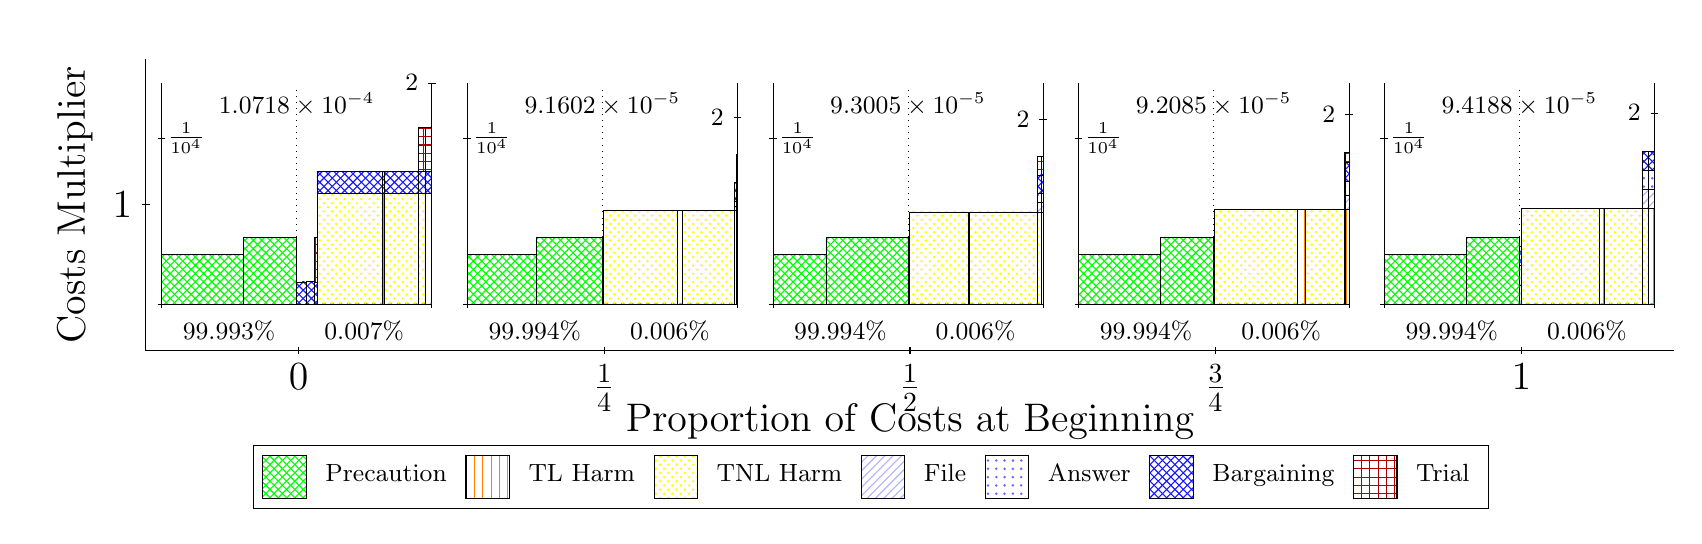
\begin{tikzpicture}
\clip(-0.5,-1.1) rectangle +(20.91,6.2);
\draw[black] (1,1) -- (1,4.7);
\node[rotate=90, fontscale=2, anchor=center] at (0.1, 2.85) {Costs Multiplier};
\draw[black] (0.95,2.85) -- (1.05,2.85);
\node[fontscale=2, anchor=east] at (0.95, 2.85) {1};

\draw[black] (1,1) -- (20.41,1);
\node[fontscale=2, anchor=center] at (10.705, 0.1) {Proportion of Costs at Beginning};
\draw[black] (2.941,0.95) -- (2.941,1.05);
\node[fontscale=2, anchor=north] at (2.941, 0.95) {0};
\draw[black] (6.823,0.95) -- (6.823,1.05);
\node[fontscale=2, anchor=north] at (6.823, 0.95) {$\frac{1}{4}$};
\draw[black] (10.705,0.95) -- (10.705,1.05);
\node[fontscale=2, anchor=north] at (10.705, 0.95) {$\frac{1}{2}$};
\draw[black] (14.587,0.95) -- (14.587,1.05);
\node[fontscale=2, anchor=north] at (14.587, 0.95) {$\frac{3}{4}$};
\draw[black] (18.469,0.95) -- (18.469,1.05);
\node[fontscale=2, anchor=north] at (18.469, 0.95) {1};


\draw[pattern=crosshatch, pattern color=green,draw=black,very thin] (1.2,1.592) rectangle (2.2435,2.2231);
\draw[pattern=crosshatch, pattern color=green,draw=black,very thin] (2.2435,1.592) rectangle (2.916,2.4334);
\draw[pattern=crosshatch, pattern color=green,draw=black,very thin] (2.916,1.592) rectangle (3.0417,1.592);
\draw[pattern=crosshatch,      pattern color=blue!90,draw=black,very thin] (2.916,1.592) rectangle (3.0417,1.8728);
\draw[pattern=crosshatch, pattern color=green,draw=black,very thin] (3.0417,1.592) rectangle (3.1425,1.5921);
\draw[pattern=crosshatch,      pattern color=blue!90,draw=black,very thin] (3.0417,1.5921) rectangle (3.1425,1.8729);
\draw[pattern=crosshatch, pattern color=green,draw=black,very thin] (3.1425,1.592) rectangle (3.1731,1.592);
\draw[pattern=crosshatch,      pattern color=blue!90,draw=black,very thin] (3.1425,1.592) rectangle (3.1731,1.8728);
\draw[pattern=grid,            pattern color=red!70!black,draw=black,very thin] (3.1425,1.8728) rectangle (3.1731,2.4344);
\draw[pattern=crosshatch, pattern color=green,draw=black,very thin] (3.1731,1.592) rectangle (3.9984,1.592);
\draw[pattern=crosshatch dots, pattern color=yellow,draw=black,very thin] (3.1731,1.592) rectangle (3.9984,2.996);
\draw[pattern=crosshatch,      pattern color=blue!90,draw=black,very thin] (3.1731,2.996) rectangle (3.9984,3.2768);
\draw[pattern=crosshatch, pattern color=green,draw=black,very thin] (3.9984,1.592) rectangle (4.0327,1.592);
\draw[pattern=vertical lines, pattern color=orange,draw=black,very thin] (3.9984,1.592) rectangle (4.0327,2.996);
\draw[pattern=crosshatch,      pattern color=blue!90,draw=black,very thin] (3.9984,2.996) rectangle (4.0327,3.2768);
\draw[pattern=crosshatch, pattern color=green,draw=black,very thin] (4.0327,1.592) rectangle (4.4588,1.5921);
\draw[pattern=crosshatch dots, pattern color=yellow,draw=black,very thin] (4.0327,1.5921) rectangle (4.4588,2.996);
\draw[pattern=crosshatch,      pattern color=blue!90,draw=black,very thin] (4.0327,2.996) rectangle (4.4588,3.2768);
\draw[pattern=crosshatch, pattern color=green,draw=black,very thin] (4.4588,1.592) rectangle (4.5436,1.592);
\draw[pattern=crosshatch dots, pattern color=yellow,draw=black,very thin] (4.4588,1.592) rectangle (4.5436,2.996);
\draw[pattern=crosshatch,      pattern color=blue!90,draw=black,very thin] (4.4588,2.996) rectangle (4.5436,3.2768);
\draw[pattern=grid,            pattern color=red!70!black,draw=black,very thin] (4.4588,3.2768) rectangle (4.5436,3.8384);
\draw[pattern=crosshatch, pattern color=green,draw=black,very thin] (4.5436,1.592) rectangle (4.632,1.592);
\draw[pattern=vertical lines, pattern color=orange,draw=black,very thin] (4.5436,1.592) rectangle (4.632,2.996);
\draw[pattern=crosshatch,      pattern color=blue!90,draw=black,very thin] (4.5436,2.996) rectangle (4.632,3.2768);
\draw[pattern=grid,            pattern color=red!70!black,draw=black,very thin] (4.5436,3.2768) rectangle (4.632,3.8384);
\node[font=\small,text=black,anchor=north] at (2.916, 4.4) {$1.0718\times 10^{-4}$};
\draw[black,very thin] (1.2,1.592) -- (1.2,4.4);
\draw[black,very thin] (1.15,1.592) -- (1.25,1.592);
\node[font=\small,text=black, anchor=west] at (1.15, 1.592) {};
\draw[black,very thin] (1.15,3.6955) -- (1.25,3.6955);
\node[font=\small,text=black, anchor=west] at (1.15, 3.6955) {$\frac{1}{10^{4}}$};

\draw[black,dotted,very thin] (2.916,1.6762) -- (2.916,4.3158);
\draw[black,very thin] (4.632,1.592) -- (4.632,4.4);
\draw[black,very thin] (4.582,4.3999) -- (4.682,4.3999);
\node[font=\small,text=black, anchor=east] at (4.582, 4.3999) {\contour{white}{2}};

\draw[black,very thin] (1.2,1.592) -- (4.632,1.592);
\draw[black,very thin] (1.2,1.542) -- (1.2,1.642);
\node[font=\small,text=black, anchor=north] at (1.2, 1.542) {};
\draw[black,very thin] (4.632,1.542) -- (4.632,1.642);
\node[font=\small,text=black, anchor=north] at (4.632, 1.542) {};

\node[font=\small,text=black,anchor=south] at (2.058, 0.992) {99.993\%};
\node[font=\small,text=black,anchor=south] at (3.774, 0.992) {0.007\%};

\draw[pattern=crosshatch, pattern color=green,draw=black,very thin] (5.082,1.592) rectangle (5.9555,2.2231);
\draw[pattern=crosshatch, pattern color=green,draw=black,very thin] (5.9555,1.592) rectangle (6.798,2.4334);
\draw[pattern=crosshatch, pattern color=green,draw=black,very thin] (6.798,1.592) rectangle (6.8027,1.592);
\draw[pattern=north east lines, pattern color=blue!30,draw=black,very thin] (6.798,1.592) rectangle (6.8027,1.6512);
\draw[pattern=dots,  pattern color=blue!60,draw=black,very thin] (6.798,1.6512) rectangle (6.8027,1.7104);
\draw[pattern=crosshatch,      pattern color=blue!90,draw=black,very thin] (6.798,1.7104) rectangle (6.8027,1.9472);
\draw[pattern=crosshatch, pattern color=green,draw=black,very thin] (6.8027,1.592) rectangle (6.8055,1.592);
\draw[pattern=north east lines, pattern color=blue!30,draw=black,very thin] (6.8027,1.592) rectangle (6.8055,1.6512);
\draw[pattern=dots,  pattern color=blue!60,draw=black,very thin] (6.8027,1.6512) rectangle (6.8055,1.7104);
\draw[pattern=crosshatch,      pattern color=blue!90,draw=black,very thin] (6.8027,1.7104) rectangle (6.8055,1.9472);
\draw[pattern=grid,            pattern color=red!70!black,draw=black,very thin] (6.8027,1.9472) rectangle (6.8055,2.3024);
\draw[pattern=crosshatch, pattern color=green,draw=black,very thin] (6.8055,1.592) rectangle (7.7449,1.592);
\draw[pattern=crosshatch dots, pattern color=yellow,draw=black,very thin] (6.8055,1.592) rectangle (7.7449,2.7759);
\draw[pattern=crosshatch, pattern color=green,draw=black,very thin] (7.7449,1.592) rectangle (7.8076,1.592);
\draw[pattern=vertical lines, pattern color=orange,draw=black,very thin] (7.7449,1.592) rectangle (7.8076,2.7759);
\draw[pattern=crosshatch, pattern color=green,draw=black,very thin] (7.8076,1.592) rectangle (8.4735,1.592);
\draw[pattern=crosshatch dots, pattern color=yellow,draw=black,very thin] (7.8076,1.592) rectangle (8.4735,2.776);
\draw[pattern=crosshatch, pattern color=green,draw=black,very thin] (8.4735,1.592) rectangle (8.4774,1.592);
\draw[pattern=crosshatch dots, pattern color=yellow,draw=black,very thin] (8.4735,1.592) rectangle (8.4774,2.7759);
\draw[pattern=north east lines, pattern color=blue!30,draw=black,very thin] (8.4735,2.7759) rectangle (8.4774,2.8351);
\draw[pattern=dots,  pattern color=blue!60,draw=black,very thin] (8.4735,2.8351) rectangle (8.4774,2.8943);
\draw[pattern=crosshatch,      pattern color=blue!90,draw=black,very thin] (8.4735,2.8943) rectangle (8.4774,3.1311);
\draw[pattern=crosshatch, pattern color=green,draw=black,very thin] (8.4774,1.592) rectangle (8.4978,1.592);
\draw[pattern=vertical lines, pattern color=orange,draw=black,very thin] (8.4774,1.592) rectangle (8.4978,2.7759);
\draw[pattern=north east lines, pattern color=blue!30,draw=black,very thin] (8.4774,2.7759) rectangle (8.4978,2.8351);
\draw[pattern=dots,  pattern color=blue!60,draw=black,very thin] (8.4774,2.8351) rectangle (8.4978,2.8943);
\draw[pattern=crosshatch,      pattern color=blue!90,draw=black,very thin] (8.4774,2.8943) rectangle (8.4978,3.1311);
\draw[pattern=crosshatch, pattern color=green,draw=black,very thin] (8.4978,1.592) rectangle (8.5058,1.592);
\draw[pattern=crosshatch dots, pattern color=yellow,draw=black,very thin] (8.4978,1.592) rectangle (8.5058,2.7759);
\draw[pattern=north east lines, pattern color=blue!30,draw=black,very thin] (8.4978,2.7759) rectangle (8.5058,2.8351);
\draw[pattern=dots,  pattern color=blue!60,draw=black,very thin] (8.4978,2.8351) rectangle (8.5058,2.8943);
\draw[pattern=crosshatch,      pattern color=blue!90,draw=black,very thin] (8.4978,2.8943) rectangle (8.5058,3.1311);
\draw[pattern=grid,            pattern color=red!70!black,draw=black,very thin] (8.4978,3.1311) rectangle (8.5058,3.4863);
\draw[pattern=crosshatch, pattern color=green,draw=black,very thin] (8.5058,1.592) rectangle (8.514,1.592);
\draw[pattern=vertical lines, pattern color=orange,draw=black,very thin] (8.5058,1.592) rectangle (8.514,2.7759);
\draw[pattern=north east lines, pattern color=blue!30,draw=black,very thin] (8.5058,2.7759) rectangle (8.514,2.8351);
\draw[pattern=dots,  pattern color=blue!60,draw=black,very thin] (8.5058,2.8351) rectangle (8.514,2.8943);
\draw[pattern=crosshatch,      pattern color=blue!90,draw=black,very thin] (8.5058,2.8943) rectangle (8.514,3.1311);
\draw[pattern=grid,            pattern color=red!70!black,draw=black,very thin] (8.5058,3.1311) rectangle (8.514,3.4863);
\node[font=\small,text=black,anchor=north] at (6.798, 4.4) {$9.1602\times 10^{-5}$};
\draw[black,very thin] (5.082,1.592) -- (5.082,4.4);
\draw[black,very thin] (5.032,1.592) -- (5.132,1.592);
\node[font=\small,text=black, anchor=west] at (5.032, 1.592) {};
\draw[black,very thin] (5.032,3.6955) -- (5.132,3.6955);
\node[font=\small,text=black, anchor=west] at (5.032, 3.6955) {$\frac{1}{10^{4}}$};

\draw[black,dotted,very thin] (6.798,1.6762) -- (6.798,4.3158);
\draw[black,very thin] (8.514,1.592) -- (8.514,4.4);
\draw[black,very thin] (8.464,3.9598) -- (8.564,3.9598);
\node[font=\small,text=black, anchor=east] at (8.464, 3.9598) {\contour{white}{2}};

\draw[black,very thin] (5.082,1.592) -- (8.514,1.592);
\draw[black,very thin] (5.082,1.542) -- (5.082,1.642);
\node[font=\small,text=black, anchor=north] at (5.082, 1.542) {};
\draw[black,very thin] (8.514,1.542) -- (8.514,1.642);
\node[font=\small,text=black, anchor=north] at (8.514, 1.542) {};

\node[font=\small,text=black,anchor=south] at (5.94, 0.992) {99.994\%};
\node[font=\small,text=black,anchor=south] at (7.656, 0.992) {0.006\%};

\draw[pattern=crosshatch, pattern color=green,draw=black,very thin] (8.964,1.592) rectangle (9.6365,2.2231);
\draw[pattern=crosshatch, pattern color=green,draw=black,very thin] (9.6365,1.592) rectangle (10.68,2.4334);
\draw[pattern=crosshatch, pattern color=green,draw=black,very thin] (10.68,1.592) rectangle (10.693,1.592);
\draw[pattern=north east lines, pattern color=blue!30,draw=black,very thin] (10.68,1.592) rectangle (10.693,1.709);
\draw[pattern=dots,  pattern color=blue!60,draw=black,very thin] (10.68,1.709) rectangle (10.693,1.826);
\draw[pattern=crosshatch,      pattern color=blue!90,draw=black,very thin] (10.68,1.826) rectangle (10.693,2.0599);
\draw[pattern=grid,            pattern color=red!70!black,draw=black,very thin] (10.68,2.0599) rectangle (10.693,2.2939);
\draw[pattern=crosshatch, pattern color=green,draw=black,very thin] (10.693,1.592) rectangle (11.446,1.592);
\draw[pattern=crosshatch dots, pattern color=yellow,draw=black,very thin] (10.693,1.592) rectangle (11.446,2.7617);
\draw[pattern=crosshatch, pattern color=green,draw=black,very thin] (11.446,1.592) rectangle (11.454,1.592);
\draw[pattern=vertical lines, pattern color=orange,draw=black,very thin] (11.446,1.592) rectangle (11.454,2.7617);
\draw[pattern=crosshatch, pattern color=green,draw=black,very thin] (11.454,1.592) rectangle (12.32,1.592);
\draw[pattern=crosshatch dots, pattern color=yellow,draw=black,very thin] (11.454,1.592) rectangle (12.32,2.7618);
\draw[pattern=crosshatch, pattern color=green,draw=black,very thin] (12.32,1.592) rectangle (12.376,1.592);
\draw[pattern=crosshatch dots, pattern color=yellow,draw=black,very thin] (12.32,1.592) rectangle (12.376,2.7617);
\draw[pattern=north east lines, pattern color=blue!30,draw=black,very thin] (12.32,2.7617) rectangle (12.376,2.8787);
\draw[pattern=dots,  pattern color=blue!60,draw=black,very thin] (12.32,2.8787) rectangle (12.376,2.9957);
\draw[pattern=crosshatch,      pattern color=blue!90,draw=black,very thin] (12.32,2.9957) rectangle (12.376,3.2296);
\draw[pattern=grid,            pattern color=red!70!black,draw=black,very thin] (12.32,3.2296) rectangle (12.376,3.4636);
\draw[pattern=crosshatch, pattern color=green,draw=black,very thin] (12.376,1.592) rectangle (12.396,1.592);
\draw[pattern=vertical lines, pattern color=orange,draw=black,very thin] (12.376,1.592) rectangle (12.396,2.7617);
\draw[pattern=north east lines, pattern color=blue!30,draw=black,very thin] (12.376,2.7617) rectangle (12.396,2.8787);
\draw[pattern=dots,  pattern color=blue!60,draw=black,very thin] (12.376,2.8787) rectangle (12.396,2.9957);
\draw[pattern=crosshatch,      pattern color=blue!90,draw=black,very thin] (12.376,2.9957) rectangle (12.396,3.2296);
\draw[pattern=grid,            pattern color=red!70!black,draw=black,very thin] (12.376,3.2296) rectangle (12.396,3.4636);
\node[font=\small,text=black,anchor=north] at (10.68, 4.4) {$9.3005\times 10^{-5}$};
\draw[black,very thin] (8.964,1.592) -- (8.964,4.4);
\draw[black,very thin] (8.914,1.592) -- (9.014,1.592);
\node[font=\small,text=black, anchor=west] at (8.914, 1.592) {};
\draw[black,very thin] (8.914,3.6955) -- (9.014,3.6955);
\node[font=\small,text=black, anchor=west] at (8.914, 3.6955) {$\frac{1}{10^{4}}$};

\draw[black,dotted,very thin] (10.68,1.6762) -- (10.68,4.3158);
\draw[black,very thin] (12.396,1.592) -- (12.396,4.4);
\draw[black,very thin] (12.346,3.9314) -- (12.446,3.9314);
\node[font=\small,text=black, anchor=east] at (12.346, 3.9314) {\contour{white}{2}};

\draw[black,very thin] (8.964,1.592) -- (12.396,1.592);
\draw[black,very thin] (8.964,1.542) -- (8.964,1.642);
\node[font=\small,text=black, anchor=north] at (8.964, 1.542) {};
\draw[black,very thin] (12.396,1.542) -- (12.396,1.642);
\node[font=\small,text=black, anchor=north] at (12.396, 1.542) {};

\node[font=\small,text=black,anchor=south] at (9.822, 0.992) {99.994\%};
\node[font=\small,text=black,anchor=south] at (11.538, 0.992) {0.006\%};

\draw[pattern=crosshatch, pattern color=green,draw=black,very thin] (12.846,1.592) rectangle (13.89,2.2231);
\draw[pattern=crosshatch, pattern color=green,draw=black,very thin] (13.89,1.592) rectangle (14.562,2.4334);
\draw[pattern=crosshatch, pattern color=green,draw=black,very thin] (14.562,1.592) rectangle (14.573,1.592);
\draw[pattern=north east lines, pattern color=blue!30,draw=black,very thin] (14.562,1.592) rectangle (14.573,1.7723);
\draw[pattern=dots,  pattern color=blue!60,draw=black,very thin] (14.562,1.7723) rectangle (14.573,1.9525);
\draw[pattern=crosshatch,      pattern color=blue!90,draw=black,very thin] (14.562,1.9525) rectangle (14.573,2.1928);
\draw[pattern=grid,            pattern color=red!70!black,draw=black,very thin] (14.562,2.1928) rectangle (14.573,2.3129);
\draw[pattern=crosshatch, pattern color=green,draw=black,very thin] (14.573,1.592) rectangle (15.622,1.592);
\draw[pattern=crosshatch dots, pattern color=yellow,draw=black,very thin] (14.573,1.592) rectangle (15.622,2.7936);
\draw[pattern=crosshatch, pattern color=green,draw=black,very thin] (15.622,1.592) rectangle (15.72,1.592);
\draw[pattern=vertical lines, pattern color=orange,draw=black,very thin] (15.622,1.592) rectangle (15.72,2.7936);
\draw[pattern=crosshatch, pattern color=green,draw=black,very thin] (15.72,1.592) rectangle (16.218,1.592);
\draw[pattern=crosshatch dots, pattern color=yellow,draw=black,very thin] (15.72,1.592) rectangle (16.218,2.7936);
\draw[pattern=crosshatch, pattern color=green,draw=black,very thin] (16.218,1.592) rectangle (16.233,1.592);
\draw[pattern=crosshatch dots, pattern color=yellow,draw=black,very thin] (16.218,1.592) rectangle (16.233,2.7936);
\draw[pattern=north east lines, pattern color=blue!30,draw=black,very thin] (16.218,2.7936) rectangle (16.233,2.9738);
\draw[pattern=dots,  pattern color=blue!60,draw=black,very thin] (16.218,2.9738) rectangle (16.233,3.154);
\draw[pattern=crosshatch,      pattern color=blue!90,draw=black,very thin] (16.218,3.154) rectangle (16.233,3.3943);
\draw[pattern=grid,            pattern color=red!70!black,draw=black,very thin] (16.218,3.3943) rectangle (16.233,3.5145);
\draw[pattern=crosshatch, pattern color=green,draw=black,very thin] (16.233,1.592) rectangle (16.278,1.592);
\draw[pattern=vertical lines, pattern color=orange,draw=black,very thin] (16.233,1.592) rectangle (16.278,2.7936);
\draw[pattern=north east lines, pattern color=blue!30,draw=black,very thin] (16.233,2.7936) rectangle (16.278,2.9738);
\draw[pattern=dots,  pattern color=blue!60,draw=black,very thin] (16.233,2.9738) rectangle (16.278,3.154);
\draw[pattern=crosshatch,      pattern color=blue!90,draw=black,very thin] (16.233,3.154) rectangle (16.278,3.3943);
\draw[pattern=grid,            pattern color=red!70!black,draw=black,very thin] (16.233,3.3943) rectangle (16.278,3.5145);
\node[font=\small,text=black,anchor=north] at (14.562, 4.4) {$9.2085\times 10^{-5}$};
\draw[black,very thin] (12.846,1.592) -- (12.846,4.4);
\draw[black,very thin] (12.796,1.592) -- (12.896,1.592);
\node[font=\small,text=black, anchor=west] at (12.796, 1.592) {};
\draw[black,very thin] (12.796,3.6955) -- (12.896,3.6955);
\node[font=\small,text=black, anchor=west] at (12.796, 3.6955) {$\frac{1}{10^{4}}$};

\draw[black,dotted,very thin] (14.562,1.6762) -- (14.562,4.3158);
\draw[black,very thin] (16.278,1.592) -- (16.278,4.4);
\draw[black,very thin] (16.228,3.995) -- (16.328,3.995);
\node[font=\small,text=black, anchor=east] at (16.228, 3.995) {\contour{white}{2}};

\draw[black,very thin] (12.846,1.592) -- (16.278,1.592);
\draw[black,very thin] (12.846,1.542) -- (12.846,1.642);
\node[font=\small,text=black, anchor=north] at (12.846, 1.542) {};
\draw[black,very thin] (16.278,1.542) -- (16.278,1.642);
\node[font=\small,text=black, anchor=north] at (16.278, 1.542) {};

\node[font=\small,text=black,anchor=south] at (13.704, 0.992) {99.994\%};
\node[font=\small,text=black,anchor=south] at (15.42, 0.992) {0.006\%};

\draw[pattern=crosshatch, pattern color=green,draw=black,very thin] (16.728,1.592) rectangle (17.772,2.2231);
\draw[pattern=crosshatch, pattern color=green,draw=black,very thin] (17.772,1.592) rectangle (18.444,2.4334);
\draw[pattern=crosshatch, pattern color=green,draw=black,very thin] (18.444,1.592) rectangle (18.471,1.592);
\draw[pattern=north east lines, pattern color=blue!30,draw=black,very thin] (18.444,1.592) rectangle (18.471,1.8345);
\draw[pattern=dots,  pattern color=blue!60,draw=black,very thin] (18.444,1.8345) rectangle (18.471,2.077);
\draw[pattern=crosshatch,      pattern color=blue!90,draw=black,very thin] (18.444,2.077) rectangle (18.471,2.3194);
\draw[pattern=crosshatch, pattern color=green,draw=black,very thin] (18.471,1.592) rectangle (19.457,1.592);
\draw[pattern=crosshatch dots, pattern color=yellow,draw=black,very thin] (18.471,1.592) rectangle (19.457,2.8044);
\draw[pattern=crosshatch, pattern color=green,draw=black,very thin] (19.457,1.592) rectangle (19.518,1.592);
\draw[pattern=vertical lines, pattern color=orange,draw=black,very thin] (19.457,1.592) rectangle (19.518,2.8044);
\draw[pattern=crosshatch, pattern color=green,draw=black,very thin] (19.518,1.592) rectangle (20.011,1.592);
\draw[pattern=crosshatch dots, pattern color=yellow,draw=black,very thin] (19.518,1.592) rectangle (20.011,2.8044);
\draw[pattern=crosshatch, pattern color=green,draw=black,very thin] (20.011,1.592) rectangle (20.079,1.592);
\draw[pattern=crosshatch dots, pattern color=yellow,draw=black,very thin] (20.011,1.592) rectangle (20.079,2.8044);
\draw[pattern=north east lines, pattern color=blue!30,draw=black,very thin] (20.011,2.8044) rectangle (20.079,3.0469);
\draw[pattern=dots,  pattern color=blue!60,draw=black,very thin] (20.011,3.0469) rectangle (20.079,3.2893);
\draw[pattern=crosshatch,      pattern color=blue!90,draw=black,very thin] (20.011,3.2893) rectangle (20.079,3.5318);
\draw[pattern=crosshatch, pattern color=green,draw=black,very thin] (20.079,1.592) rectangle (20.16,1.592);
\draw[pattern=vertical lines, pattern color=orange,draw=black,very thin] (20.079,1.592) rectangle (20.16,2.8044);
\draw[pattern=north east lines, pattern color=blue!30,draw=black,very thin] (20.079,2.8044) rectangle (20.16,3.0469);
\draw[pattern=dots,  pattern color=blue!60,draw=black,very thin] (20.079,3.0469) rectangle (20.16,3.2893);
\draw[pattern=crosshatch,      pattern color=blue!90,draw=black,very thin] (20.079,3.2893) rectangle (20.16,3.5318);
\node[font=\small,text=black,anchor=north] at (18.444, 4.4) {$9.4188\times 10^{-5}$};
\draw[black,very thin] (16.728,1.592) -- (16.728,4.4);
\draw[black,very thin] (16.678,1.592) -- (16.778,1.592);
\node[font=\small,text=black, anchor=west] at (16.678, 1.592) {};
\draw[black,very thin] (16.678,3.6955) -- (16.778,3.6955);
\node[font=\small,text=black, anchor=west] at (16.678, 3.6955) {$\frac{1}{10^{4}}$};

\draw[black,dotted,very thin] (18.444,1.6762) -- (18.444,4.3158);
\draw[black,very thin] (20.16,1.592) -- (20.16,4.4);
\draw[black,very thin] (20.11,4.0167) -- (20.21,4.0167);
\node[font=\small,text=black, anchor=east] at (20.11, 4.0167) {\contour{white}{2}};

\draw[black,very thin] (16.728,1.592) -- (20.16,1.592);
\draw[black,very thin] (16.728,1.542) -- (16.728,1.642);
\node[font=\small,text=black, anchor=north] at (16.728, 1.542) {};
\draw[black,very thin] (20.16,1.542) -- (20.16,1.642);
\node[font=\small,text=black, anchor=north] at (20.16, 1.542) {};

\node[font=\small,text=black,anchor=south] at (17.586, 0.992) {99.994\%};
\node[font=\small,text=black,anchor=south] at (19.302, 0.992) {0.006\%};

\coordinate (LegendAnchor) at (10.205000000000002,0);
\begin{scope}[align=center]
\matrix[scale=0.6,draw=black,below=0.2cm of LegendAnchor,nodes={draw},column sep=0.12cm]{
\node[rectangle,draw,minimum width=0.55cm,minimum height=0.55cm,pattern=crosshatch, pattern color=green]{}; &
        \node[draw=none,font=\small]{Precaution}; &
\node[rectangle,draw,minimum width=0.55cm,minimum height=0.55cm,pattern=vertical lines, pattern color=orange]{}; &
        \node[draw=none,font=\small]{TL Harm}; &
\node[rectangle,draw,minimum width=0.55cm,minimum height=0.55cm,pattern=crosshatch dots, pattern color=yellow]{}; &
        \node[draw=none,font=\small]{TNL Harm}; &
\node[rectangle,draw,minimum width=0.55cm,minimum height=0.55cm,pattern=north east lines, pattern color=blue!30]{}; &
        \node[draw=none,font=\small]{File}; &
\node[rectangle,draw,minimum width=0.55cm,minimum height=0.55cm,pattern=dots, pattern color=blue!60]{}; &
        \node[draw=none,font=\small]{Answer}; &
\node[rectangle,draw,minimum width=0.55cm,minimum height=0.55cm,pattern=crosshatch, pattern color=blue!90]{}; &
        \node[draw=none,font=\small]{Bargaining}; &
\node[rectangle,draw,minimum width=0.55cm,minimum height=0.55cm,pattern=grid, pattern color=red!70!black]{}; &
        \node[draw=none,font=\small]{Trial}; \\
};\end{scope}

\end{tikzpicture}
\end{document}